\begin{flushright} {\tiny {\color{gray} diff1D.tex}} \end{flushright}

Let us consider the following one-dimensional grid: 
\begin{center}
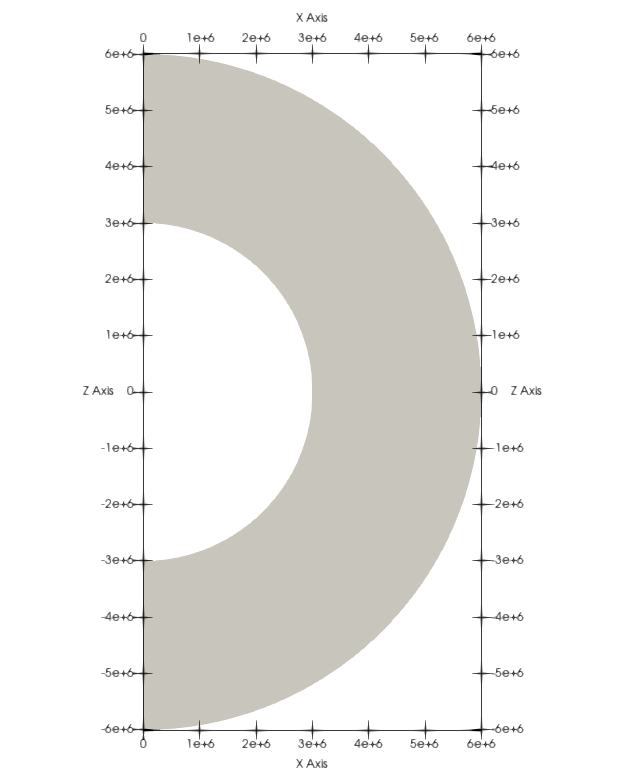
\includegraphics[width=10cm]{images/oneD/domain}
\end{center}
Its spans the domain $\Omega$ of length $L_x$. 
It is discretised by means of 
$nnx$ nodes and $nelx=nnx-1$ elements.
Zooming in on the element $e$ which is bounded by two nodes $k$ and $k+1$,
its size (also sometimes called diameter) is $h_x=x_{k+1}-x_k$, 
and the temperature field we wish to compute is located on those 
nodes so that they are logically called $T_k$ and $T_{k+1}$:

\begin{center}
\includegraphics[width=8cm]{images/oneD/el1D}
\end{center}

\begin{remark}
In what follows I will indicate 
mathematical functions\footnote{\url{https://en.wikipedia.org/wiki/Function_(mathematics)}} 
by this {\color{violet} color}.
\end{remark}

\begin{remark}
In what follows $\int_{\Omega_e}$ should be understood as $\int_{x_k}^{x_{k+1}}$.
\end{remark}


%........................................................
\subsubsection{From the strong form to the weak form}

We focus here on the 1D diffusion equation (no advection, no heat sources, see Section~\ref{ss:hte}):
\begin{equation}
\rho C_p \frac{\partial {\color{violet}T}}{\partial t} 
= \frac{\partial }{\partial x} \left( k \frac{\partial {\color{violet}T}}{\partial x}  \right)
\end{equation}
where $\rho$ is the density, $C_p$ the heat capacity and $k$ the heat conductivity. All three coefficients
are assumed to be constant in space and time.

This is the {\color{olive}strong form} of the PDE to solve. \index{general}{Strong Form}
I can multiply this equation by a function\footnote{This function should be well-behaved with 
special properties, but we here assume it is a polynomial function.} ${\color{violet}f}(x)$ 
and integrate it over $\Omega$:
\begin{equation}
\int_{\Omega} {\color{violet}f}(x) \;  \rho C_p\frac{\partial {\color{violet}T}}{\partial t} dx
=
\int_{\Omega} {\color{violet}f}(x) \;  \frac{\partial }{\partial x} \left( k \frac{\partial {\color{violet}T}}{\partial x}  \right) dx
\end{equation}
Looking at the right hand side, it is of the form $\int u v'$ so that I 
integrate it by parts\footnote{$\int_\Omega uv' = \int_{\partial\Omega} uv - \int_\Omega u'v$}:
\begin{equation}
\int_{\Omega} {\color{violet}f}(x) \;  \frac{\partial }{\partial x} 
\left( k \frac{\partial {\color{violet}T}}{\partial x}  \right) dx
=
\left[
 {\color{violet}f}(x) \;  k \frac{\partial {\color{violet}T}}{\partial x}
\right]_{\partial \Omega}
-
\int_{\Omega} \frac{\partial {\color{violet}f}}{\partial x} \;   k \frac{\partial {\color{violet}T}}{\partial x}  dx
\end{equation}
Assuming there is no heat flux on the boundary\footnote{This is of course not always the case
and we will revisit this at a later stage in the course.} (i.e. $q_x= - k \partial {\color{violet}T}/\partial x = 0$ ), then
\begin{equation}
\int_{\Omega} {\color{violet}f}(x) \frac{\partial }{\partial x} \left( k \frac{\partial {\color{violet}T}}{\partial x}  
\right) dx
=
- \int_{\Omega} \frac{\partial {\color{violet}f}}{\partial x}  k \frac{\partial {\color{violet}T}}{\partial x}  dx
\end{equation}
We then obtain the {\color{olive}weak form} of the diffusion equation in 1D:
\begin{equation}
\boxed{
\int_{\Omega} {\color{violet}f}(x) \rho C_p \frac{\partial {\color{violet}T}}{\partial t} dx
+
\int_{\Omega} \frac{\partial {\color{violet}f}}{\partial x}  k \frac{\partial {\color{violet}T}}{\partial x}  dx = 0
}
\end{equation}
We then use the additive property of the integral 
$\int_\Omega \dots = \sum\limits_{elts} \int_{\Omega_e} \dots$
so that the equation above becomes 
\begin{equation}
\sum_{elts} \left(     
\underbrace{ \int_{\Omega_e} {\color{violet}f}(x) \rho C_p   \frac{\partial {\color{violet}T}}{\partial t} dx }_{{\Lambda}_f^e}
+
\underbrace{\int_{\Omega_e} \frac{\partial {\color{violet}f}}{\partial x}  k \frac{\partial {\color{violet}T}}{\partial x}  dx}_{{\Upsilon}_f^e}      \right) = 0  
\end{equation}


%........................................................
\subsubsection{From the weak form to a linear system}

In order to compute these integrals (analytically or by means of a numerical quadrature), 
we will need to evaluate ${\color{violet}T}$ inside the element. However, inside the element, 
the temperature is not known: all we hope to have at some point is the temperature at the nodes (
this is what the code will compute). 

For $x\in [x_k,x_{k+1}]$ we need to come up with a way to formulate the temperature in this element and 
we coin this ${\color{violet}T}^h$.  
It makes sense to think that ${\color{violet}T}^h(x)$ will then be a function of the temperature at the nodes, 
i.e. ${\color{violet}T}^h(x) = \alpha T_k + \beta T_{k+1}$ where $\alpha$ and $\beta$ are coefficients. 
One over-simplified approach would be to assign ${\color{violet}T}^h(x)=(T_k + T_{k+1})/2$ 
(i.e. ${\color{violet}T^h}$ is a zero-th order polynomial) but this would make the
temperature discontinuous from element to element so we discard this option. 
A rather logical and simple solution to this problem is a linear temperature field between $T_k$
and $T_{k+1}$: 

\begin{eqnarray}
{\color{violet}T}^h(x) 
%&=& N_{k}(x) T_k + N_{k+1}(x) T_{k+1}  \nn\\
&=& \underbrace{\frac{x_{k+1}-x}{h_x}}_{{\color{violet}\bN}_k^\uptheta(x)} T_k 
+ 
\underbrace{\frac{x-x_k}{h_x}}_{{\color{violet}\bN}_{k+1}^\uptheta(x)} T_{k+1} \nn
\end{eqnarray}
where ${\color{violet}\bN}_k^\uptheta(x)$ is the (temperature) basis function associated to node $k$ and 
${\color{violet}\bN}_{k+1}^\uptheta(x)$ is the basis function associated to node $k+1$.

Rather reassuringly, we have:
\begin{itemize}
\item $x=x_k$ yields ${\color{violet}T}^h(x_k)=T_k$
\item $x=x_{k+1}$ yields ${\color{violet}T}^h(x_{k+1})=T_{k+1}$
\item $x=x_{1/2}=(x_k+x_{k+1})/2$ yields ${\color{violet}T}^h(x_{1/2})=(T_k+T_{k+1})/2$
\end{itemize}
In what follows we abbreviate $\partial {\color{violet}T}^h/\partial t$ by $\dot{\color{violet}T}^h(x)$.
Let us compute ${\Lambda}_f^e$ and ${\Upsilon}_f^e$ separately.
\begin{eqnarray}
{\Lambda}_f^e 
&=&\int_{x_k}^{x_{k+1}} {\color{violet}f}(x) \rho C_p \dot {\color{violet}T}^h(x) dx \nn\\
&=& \int_{x_k}^{x_{k+1}} {\color{violet}f}(x) \rho C_p \;\;  [ {\color{violet}\bN}_{k}^\uptheta(x) \dot{T}_k 
+ {\color{violet}\bN}_{k+1}^\uptheta(x) \dot{T}_{k+1} ] \;\; dx  \nn\\
&=& \int_{x_k}^{x_{k+1}} {\color{violet}f}(x) \rho C_p {\color{violet}\bN}_{k}^\uptheta(x) \dot{T}_k  dx  
+ \int_{x_k}^{x_{k+1}} {\color{violet}f}(x) 
\rho C_p {\color{violet}\bN}_{k+1}^\uptheta(x) \dot{T}_{k+1}   dx \nn\\
&=&  \left( \int_{x_k}^{x_{k+1}} {\color{violet}f}(x) \rho C_p  
{\color{violet}\bN}_{k}^\uptheta(x) dx \right) \dot{T}_k  
+ \left( \int_{x_k}^{x_{k+1}} {\color{violet}f}(x) \rho C_p 
{\color{violet}\bN}_{k+1}^\uptheta(x) dx \right)  \dot{T}_{k+1}  \nn
\end{eqnarray}
Taking ${\color{violet}f}(x)={\color{violet}\bN}_k^\uptheta(x)$ and omitting '$(x)$' in the rhs:
\[
{\Lambda}_{\bN_k^\uptheta}^e=
%\int_{x_k}^{x_{k+1}} {\color{blue}f}(x) \rho C_p \dot{\color{blue}T}(x) dx
\left( \int_{x_k}^{x_{k+1}} \rho C_p  {\color{violet}\bN}_k^\uptheta 
{\color{violet}\bN}_{k}^\uptheta dx \right) \dot{T}_k  
+ \left( \int_{x_k}^{x_{k+1}} \rho C_p {\color{violet}\bN}_k^\uptheta 
{\color{violet}\bN}_{k+1}^\uptheta dx \right)  \dot{T}_{k+1} 
\]
Taking ${\color{violet}f}(x)={\color{violet}\bN}_{k+1}^\uptheta(x)$ 
and omitting '$(x)$' in the rhs:
\[
{\Lambda}_{\bN_{k+1}^\uptheta}^e
%\int_{x_k}^{x_{k+1}} {\color{blue}f}(x) \dot{\color{blue}T}(x) dx
= \left( \int_{x_k}^{x_{k+1}} \rho C_p {\color{violet}\bN}_{k+1}^\uptheta 
{\color{violet}N}_{k}^\uptheta dx \right) \dot{T}_k  
+ \left( \int_{x_k}^{x_{k+1}} \rho C_p {\color{violet}\bN}_{k+1}^\uptheta 
{\color{violet}N}_{k+1}^\uptheta dx \right)  \dot{T}_{k+1} 
\]
We can rearrange these last two equations as follows:
\[
\left(
\begin{array}{c}
{\Lambda}_{\bN_k^\uptheta}^e  \\ \\ 
{\Lambda}_{\bN_{k+1}^\uptheta}^e
\end{array}
\right)
=
\left(
\begin{array}{cc}
\int_{x_k}^{x_{k+1}} {\color{violet}\bN}_k^\uptheta        \rho C_p {\color{violet}\bN}_{k}^\uptheta dx  
&  \int_{x_k}^{x_{k+1}} {\color{violet}\bN}_k^\uptheta     \rho C_p {\color{violet}\bN}_{k+1}^\uptheta dx\\ \\
\int_{x_k}^{x_{k+1}} {\color{violet}\bN}_{k+1}^\uptheta    \rho C_p {\color{violet}\bN}_{k}^\uptheta dx  
&  \int_{x_k}^{x_{k+1}} {\color{violet}\bN}_{k+1}^\uptheta \rho C_p {\color{violet}\bN}_{k+1}^\uptheta dx 
\end{array}
\right)
\cdot
\left(
\begin{array}{c}
\dot{T}_k \\ \\
\dot{T}_{k+1}
\end{array}
\right)
\]
and we can take the integrals outside of the matrix:
\[
\left(
\begin{array}{c}
{\Lambda}_{\bN_k^\uptheta}^e \\ \\ {\Lambda}_{\bN_{k+1}^\uptheta}^e
\end{array}
\right)
=
\left[
\int_{x_k}^{x_{k+1}}
\rho C_p
\left(
\begin{array}{cc}
{\color{violet}N}_k^\uptheta     {\color{violet}\bN}_{k}^\uptheta 
&  {\color{violet}\bN}_k^\uptheta     {\color{violet}N}_{k+1}^\uptheta  \\ \\
{\color{violet}N}_{k+1}^\uptheta {\color{violet}\bN}_{k}^\uptheta 
&  {\color{violet}\bN}_{k+1}^\uptheta {\color{violet}N}_{k+1}^\uptheta 
\end{array}
\right)
dx
\right]
\cdot
\left(
\begin{array}{c}
\dot{T}_k \\ \\ 
\dot{T}_{k+1}
\end{array}
\right)
\]
Finally, we can define the vectors 
\[
{\vec {\color{violet}\bN}}^T = 
\left(
\begin{array}{c}
{\color{violet}\bN}_k^\uptheta(x)  \\ \\  {\color{violet}\bN}_{k+1}^\uptheta (x)
\end{array}
\right)
\]
and 
\[
{\vec T}^e = 
\left(
\begin{array}{c}
T_k \\ \\ T_{k+1}
\end{array}
\right)
\quad
\quad
\quad
\quad
\quad
\dot{\vec T}^e = 
\left(
\begin{array}{c}
\dot{T}_k \\ \\ \dot{T}_{k+1}
\end{array}
\right)
\]
so that 
\[
\left(
\begin{array}{c}
{\Lambda}_{\bN_k^\uptheta}^e \\  \\ 
{\Lambda}_{\bN_{k+1}^\uptheta}^e
\end{array}
\right)
=
\left( \int_{x_k}^{x_{k+1}}   
{\vec {\color{violet}\bN}}^T \rho C_p  {\vec {\color{violet}\bN}} dx  \right) \cdot \dot{\vec T}^e
\]
Let us now go back to the diffusion term:
\begin{eqnarray}
{\Upsilon}_f^e &=&
\int_{x_k}^{x^{k+1}} \frac{\partial {\color{violet}f}}{\partial x} k 
\frac{\partial {\color{violet}T}^h}{\partial x} dx \nn\\
&=&
\int_{x_k}^{x^{k+1}} \frac{\partial {\color{violet}f}}{\partial x} k \frac{\partial  
({\color{violet}\bN}_{k}^\uptheta(x) T_k 
+ {\color{violet}\bN}_{k+1}^\uptheta(x) T_{k+1} ) }{\partial x} dx  \nn\\
%&=&
%\int_{x_k}^{x^{k+1}} \left( \frac{\partial {\color{blue}f}}{\partial x}  \frac{\partial  {\color{blue}N}_{k} } {\partial x}  T_k 
%+ \frac{\partial {\color{blue}f}}{\partial x}  \frac{\partial  {\color{blue}N}_{k+1} } {\partial x}  T_{k+1} \right)  dx \nn\\
&=&
\left( \int_{x_k}^{x^{k+1}} \frac{\partial {\color{violet}f}}{\partial x}  
k \frac{\partial  {\color{violet}\bN}_{k}^\uptheta } {\partial x}  dx \right)  T_k 
+ \left( \int_{x_k}^{x^{k+1}} \frac{\partial {\color{violet}f}}{\partial x}  
k \frac{\partial  {\color{violet}\bN}_{k+1}^\uptheta } {\partial x} dx \right) T_{k+1}  \nn
\end{eqnarray}
Taking ${\color{violet}f}(x)={\color{violet}\bN}_k^\uptheta(x)$ 
\[
{\Upsilon}_{\bN_k^\uptheta}^e=
%\int_{x_k}^{x^{k+1}} \frac{\partial {\color{blue}f}}{\partial x} \frac{\partial {\color{blue}T}}{\partial x} dx
\left( \int_{x_k}^{x^{k+1}} k\frac{\partial {\color{violet}\bN}_k^\uptheta}{\partial x}  
\frac{\partial  {\color{violet}\bN}_{k}^\uptheta } {\partial x}  dx \right)  T_k 
+ \left( \int_{x_k}^{x^{k+1}} k\frac{\partial {\color{violet}\bN}_k^\uptheta}{\partial x}  
\frac{\partial  {\color{violet}\bN}_{k+1}^\uptheta } {\partial x} dx \right) T_{k+1}  \nn
\]
Taking ${\color{violet}f}(x)={\color{violet}\bN}_{k+1}^\theta(x)$ 
\[
{\Upsilon}_{\bN_{k+1}^\uptheta}^e=
%\int_{x_k}^{x^{k+1}} \frac{\partial {\color{blue}f}}{\partial x} \frac{\partial {\color{blue}T}}{\partial x} dx
%=
\left( \int_{x_k}^{x^{k+1}} k\frac{\partial {\color{violet}\bN}_{k+1}^\uptheta}{\partial x}  
\frac{\partial  {\color{violet}\bN}_{k}^\uptheta } {\partial x}  dx \right)  T_k 
+ 
\left( \int_{x_k}^{x^{k+1}} k\frac{\partial {\color{violet}\bN}_{k+1}^\uptheta}{\partial x}  
\frac{\partial  {\color{violet}\bN}_{k+1}^\uptheta } {\partial x} dx \right) T_{k+1}  \nn
\]


\[
\left(
\begin{array}{cc}
{\Upsilon}_{\bN_k^\uptheta}^e \\ \\ 
{\Upsilon}_{\bN_{k+1}^\uptheta}^e
\end{array}
\right)
=
\left(
\begin{array}{cc}
\int_{x_k}^{x^{k+1}} \frac{\partial {\color{violet}\bN}_k^\uptheta}{\partial x} 
k \frac{\partial  {\color{violet}\bN}_{k}^\uptheta } {\partial x}  dx & 
\int_{x_k}^{x^{k+1}} \frac{\partial {\color{violet}\bN}_k^\uptheta}{\partial x} 
k \frac{\partial  {\color{violet}\bN}_{k+1}^\uptheta } {\partial x} dx 
\\ \\
\int_{x_k}^{x^{k+1}} \frac{\partial {\color{violet}\bN}_{k+1}^\uptheta}{\partial x} 
k \frac{\partial  {\color{violet}\bN}_{k}^\uptheta } {\partial x}  dx & 
\int_{x_k}^{x^{k+1}} \frac{\partial {\color{violet}\bN}_{k+1}^\uptheta}{\partial x} 
k \frac{\partial  {\color{violet}\bN}_{k+1}^\uptheta } {\partial x} dx 
\end{array}
\right)
\cdot
\left(
\begin{array}{c}
T_k \\ \\ T_{k+1}
\end{array}
\right)
\]

or,
\[
\left(
\begin{array}{cc}
{\Upsilon}_{\bN_k^\uptheta}^e \\ \\ 
{\Upsilon}_{\bN_{k+1}^\uptheta}^e
\end{array}
\right)
=
\left[
\int_{x_k}^{x^{k+1}}
k
\left(
\begin{array}{cc}
\frac{\partial {\color{violet}\bN}_k^\uptheta}{\partial x}  \frac{\partial  
{\color{violet}\bN}_{k}^\uptheta } {\partial x}   & 
\frac{\partial {\color{violet}\bN}_k^\uptheta}{\partial x}  \frac{\partial  
{\color{violet}\bN}_{k+1}^\uptheta } {\partial x}  
\\ \\
\frac{\partial {\color{violet}\bN}_{k+1}^\uptheta}{\partial x}  \frac{\partial  
{\color{violet}\bN}_{k}^\uptheta } {\partial x}   & 
\frac{\partial {\color{violet}\bN}_{k+1}^\uptheta}{\partial x}  \frac{\partial  
{\color{violet}\bN}_{k+1}^\uptheta } {\partial x}  
\end{array}
\right)
dx
\right]
\cdot
\left(
\begin{array}{c}
T_k \\ \\ T_{k+1}
\end{array}
\right)
\]
Finally, we can define the vector 
\[
{\vec {\color{violet}B}}^T=
\left(
\begin{array}{cc}
\frac{\partial {\color{violet}\bN}_k^\uptheta}{\partial x}   \\ \\
\frac{\partial {\color{violet}\bN}_{k+1}^\uptheta}{\partial x}
\end{array}
\right)
\]
so that 
\[
\left(
\begin{array}{cc}
{\Upsilon}_{\bN_k^\uptheta}^e \\ \\ 
{\Upsilon}_{\bN_{k+1}^\uptheta}^e
\end{array}
\right)
=
\left( \int_{x_k}^{x_{k+1}}   {\vec {\color{violet}B}}^T 
k {\vec {\color{violet}B}} dx  \right) \cdot {\vec T}^e
\]

The weak form discretised over 1 element becomes
\[
\underbrace{\left( \int_{x_k}^{x_{k+1}}   {\vec {\color{violet}\bN}}^T 
\rho C_p {\vec {\color{violet}\bN}} dx  \right) }_{\bm M^e} \cdot \dot{\vec T}^e
+
\underbrace{\left( \int_{x_k}^{x_{k+1}}   {\vec {\color{violet}B}}^T k 
{\vec {\color{violet}B}} dx  \right)}_{{\bm K}_d^e} \cdot {\vec T}^e
=0
\]
or,
\[
\boxed{
{\bm M}^e \cdot \dot{\vec T}^e + {\bm K}_d^e \cdot {\vec T}^e = 0
}
\]
or,
\[
\boxed{
{\bm M}^e \cdot \frac{\partial {\vec T}^e}{\partial t} + {\bm K}_d^e \cdot {\vec T}^e = 0
}
\]
${\bm M}^e$ is commonly called the {\color{olive}mass matrix}, or capacitance matrix \cite[p103]{reddybook2}.
Note that the matrices are not coloured: the $x$ dependence has disappeared when 
the integration was carried out.
\index{general}{Mass Matrix}\index{general}{Capacitance Matrix}



In what follows I will omit the $e$ superscript on the $\vec{T}$ term to simplify notations. 

We use a first order in time discretisation for the time derivative:
\[
\dot{\vec T}= \frac{\partial {\vec T}}{\partial t} = \frac{{\vec T}^{new}-{\vec T}^{old}}{\delta t}
\]
and in the context of an implicit scheme we get
\[
{\bm M}^e \cdot \frac{{\vec T}^{new}-{\vec T}^{old}}{\delta t} + {\bm K}_d^e \cdot {\vec T}^{new} = 0
\]
or, 
\[
\boxed{
( {\bm M}^e +  {\bm K}_d^e  \delta t ) \cdot {\vec T}^{new} =  {\bm M}^e \cdot  {\vec T}^{old}
}
\]
with 
\[
{\bm M}^e=  \int_{x_k}^{x_{k+1}}   {\vec {\color{violet}\bN}}^T \rho C_p {\vec {\color{violet}\bN}} dx  
\quad\quad\quad
{\bm K}_d^e =
 \int_{x_k}^{x_{k+1}}   {\vec {\color{violet}B}}^T k {\vec {\color{violet}B}} dx 
\]

%........................................................
\subsubsection{Computing the elemental matrices}

Let us compute ${\bm M}^e$ for an element:
\[
{\bm M}^e
= \int_{x_k}^{x_{k+1}}   {\vec {\color{violet}\bN}}^T \rho C_p {\vec {\color{violet}\bN}} dx  
=
\left(
\begin{array}{cc}
\int_{x_k}^{x_{k+1}} \rho C_p {\color{violet}\bN}_k^\uptheta {\color{violet}\bN}_{k}^\uptheta dx   
&  \int_{x_k}^{x_{k+1}} \rho C_p {\color{violet}\bN}_k^\uptheta {\color{violet}\bN}_{k+1}^\uptheta dx \\ \\
\int_{x_k}^{x_{k+1}} \rho C_p {\color{violet}\bN}_{k+1}^\uptheta {\color{violet}\bN}_{k}^\uptheta dx  
&  \int_{x_k}^{x_{k+1}} \rho C_p {\color{violet}\bN}_{k+1}^\uptheta {\color{violet}\bN}_{k+1}^\uptheta dx 
\end{array}
\right)
=
\left(
\begin{array}{cc}
M_{11} & M_{12} \\
M_{21} & M_{22} 
\end{array}
\right)
\]
with 
\[
{\vec {\color{violet}\bN}}^T = 
\left(
\begin{array}{c}
{\color{violet}\bN}_k^\uptheta(x)  \\ \\  
{\color{violet}\bN}_{k+1}^\uptheta(x)
\end{array}
\right)
=
\left(
\begin{array}{c}
\frac{x_{k+1}-x}{h_x}   \\ \\
\frac{x-x_k}{h_x} 
\end{array}
\right)
\]
We only need to compute 3 integrals since $M_{12}=M_{21}$.
Let us start with $M_{11}$:
\[
M_{11}=\int_{x_k}^{x_{k+1}} \rho C_p {\color{violet}\bN}_k^\uptheta(x) 
{\color{violet}\bN}_{k}^\uptheta(x) dx
=   
\int_{x_k}^{x_{k+1}} \rho C_p 
\frac{x_{k+1}-x}{h_x}  
\frac{x_{k+1}-x}{h_x}  
dx
\]
It is then customary to carry out the change of variable $x \rightarrow r$ where 
$r \in [-1:1]$ as shown hereunder:
\begin{center}
\includegraphics[width=10cm]{images/oneD/el1D_mapping}
\end{center}
The relationships between $x$ and $r$ are:
\[
r=\frac{2}{h_x}(x-x_k)-1
\quad\quad\quad
x=\frac{h_x}{2}(1+r)+x_k
\]
In what follows we assume for simplicity that $\rho$ and $C_p$ are constant within each element so that:
\[
M_{11}=
\rho C_p
\int_{\tiny x_k}^{x_{k+1}} 
\frac{x_{k+1}-x}{h_x}  
\frac{x_{k+1}-x}{h_x}  
dx
%=  \rho C_p \int_{-1}^{+1} \frac{1}{2}(1-r) \frac{1}{2}(1-r)  \frac{h_x}{2} dr  = \frac{h_x}{3} \rho C_p \nn
=  \frac{\rho C_p h_x}{8} \int_{-1}^{+1} (1-r) (1-r)  dr  = \rho C_p \frac{h_x}{3} 
\]
Similarly we arrive at 
\begin{eqnarray}
M_{12}
&=&\rho C_p 
\int_{x_k}^{x_{k+1}} 
\frac{x_{k+1}-x}{h_x}  
\frac{x-x_k}{h_x}  
dx
=
\frac{\rho C_p  h_x}{8} 
\int_{-1}^{+1} (1-r) (1+r)dr
= \rho C_p\frac{h_x}{6}  \nn\\
M_{22}
&=&
\rho C_p 
\int_{x_k}^{x_{k+1}} 
\frac{x-x_k}{h_x}  
\frac{x-x_k}{h_x}  
dx
=
\frac{\rho C_p  h_x}{8} 
\int_{-1}^{+1} (1+r) (1+r)dr
= \rho C_p \frac{h_x}{3} \nn 
\end{eqnarray}
Finally 
\[
\boxed{
{\bm M}^e= \rho C_p \frac{h_x}{3}   
\left(
\begin{array}{cc}
1  & 1/2 \\
1/2 & 1
\end{array}
\right)
}
\]
In the new coordinate system, the {\color{olive}basis functions} 
\[
{\color{violet}\bN}_k^\uptheta(x) = \frac{x_{k+1}-x}{h_x} 
\quad
\quad
\quad
{\color{violet}\bN}_{k+1}^\uptheta(x) = \frac{x-x_k}{h_x} 
\]
become 
\[
{\color{violet}\bN}_k^\uptheta(r) = \frac{1}{2} (1-r)
\quad
\quad
\quad
{\color{violet}\bN}_{k+1}^\uptheta(r) = \frac{1}{2} (1+r)
\]
Also, 
\[
\frac{\partial {\color{violet}\bN}_k^\uptheta}{\partial x} = - \frac{1}{h_x} 
\quad
\quad
\quad
\frac{\partial {\color{violet}\bN}_{k+1}^\uptheta}{\partial x} = \frac{1}{h_x} 
\]
so that 
\[
{\vec {\color{violet}B}}^T=
\left(
\begin{array}{cc}
 \frac{\partial {\color{violet}\bN}_k^\uptheta}{\partial x}   \\ \\
 \frac{\partial {\color{violet}\bN}_{k+1}^\uptheta}{\partial x}
\end{array}
\right)
=
\left(
\begin{array}{cc}
-\frac{1}{h_x} \\ \\
\frac{1}{h_x} 
\end{array}
\right)
\]
We here also assume that the heat conductivity $k$ is constant within the element:
\[
{\bm K}_d^e =
\int_{x_k}^{x_{k+1}}   {\vec {\color{violet}B}}^T k {\vec {\color{violet}B}} dx 
= k \int_{x_k}^{x_{k+1}}   {\vec {\color{violet}B}}^T {\vec {\color{violet}B}} dx 
\]
simply becomes
\[
{\bm K}_d^e = k
 \int_{x_k}^{x_{k+1}} 
\frac{1}{h_x^2}
\left(
\begin{array}{cc}
1 & -1 \\ -1 & 1
\end{array}
\right)
dx
\]
and then
\[
\boxed{
{\bm K}_d^e =
\frac{k}{h_x}
\left(
\begin{array}{cc}
1 & -1 \\ -1 & 1
\end{array}
\right)
}
\]

%.........................................................................
\subsubsection{In practice}

Let us consider this very simple grid consisting of 4 elements/5 nodes\footnote{I have here adopted the illogical 
numbering of python -- the language used by my students-- 
so that python programmers can benchmark their code against this simple example}:
\begin{center}
\includegraphics[width=10cm]{images/oneD/grid5}
\end{center}
For each element we have 
\[
\underbrace{( {\bm M}^e +  {\bm K}_d^e \; \delta t )}_{\bm A^{e}} \cdot {\vec T}^{new} =  
\underbrace{{\bm M}^e \cdot  {\vec T}^{old} }_{\vec b^{e}}
\]
with 
\[
\vec{T}^{new}=
\left(
\begin{array}{c}
T_k^{new} \\ T_{k+1}^{new}
\end{array}
\right)
\]
We can write this equation very explicitely for each element:
\begin{itemize}
\item \underline{element {\color{red}\tt 0}}
\[
{\bm A}^{\color{red} \tt 0}  \cdot 
\left(
\begin{array}{c}
T_0^{new} \\ T_1^{new}
\end{array}
\right)
 =  {\vec b}^{\color{red} \tt 0}
\qquad
\rightarrow
\qquad
\left\{ 
\begin{array}{l}
A_{00}^{{\color{red}\tt 0}} T_0^{new} + A_{01}^{{\color{red}\tt 0}} T_1^{new} = b^{{\color{red} \tt 0}}_0 \\
A_{10}^{{\color{red}\tt 0}} T_0^{new} + A_{11}^{{\color{red}\tt 0}} T_1^{new} = b^{{\color{red} \tt 0}}_1
\end{array}
\right.
\]
Element {\color{red}\tt 0} is made of nodes 0 and 1, so it will contributes to lines and columns 0,1 of the FE matrix:
\[
\left( \begin{array}{ccccc}
A_{00}^{{\color{red}\tt 0}} &  A_{01}^{{\color{red}\tt 0}} &0&0&0 \\ 
A_{10}^{{\color{red}\tt 0}} &  A_{11}^{{\color{red} \tt 0}}  &0  &0&0 \\
0 & 0 & 0 & 0 & 0 \\ 
0 & 0 & 0 & 0 & 0 \\ 
0 & 0 & 0 & 0 & 0 
\end{array} \right) \cdot
\left(\begin{array}{c}
T_0^{new} \\ T_1^{new} \\ T_2^{new} \\ T_3^{new} \\ T_4^{new}
\end{array} \right)
=
\left(\begin{array}{c}
b_{0}^{{\color{red}\tt 0}} \\  b_{1}^{{\color{red}\tt 0}} \\  0 \\  0 \\ 0
\end{array}\right)
\]





\item \underline{element {\color{red}\tt 1}} 
\[
{\bm A}^{\color{red} \tt 1}  \cdot 
\left(
\begin{array}{c}
T_1^{new} \\ T_2^{new}
\end{array}
\right)
 =  {\vec b}^{\color{red} \tt 1}
\qquad
\rightarrow
\qquad
\left\{ 
\begin{array}{l}
A_{00}^{{\color{red}\tt 1}} T_1^{new} + A_{01}^{{\color{red}\tt 1}} T_2^{new} = b^{{\color{red} \tt 1}}_0 \\
A_{10}^{{\color{red}\tt 1}} T_1^{new} + A_{11}^{{\color{red}\tt 1}} T_2^{new} = b^{{\color{red} \tt 1}}_1
\end{array}
\right.
\]
Element {\color{red}\tt 1} is made of nodes 1 and 2, so it will contributes to lines and columns 1,2 of the FE matrix:
\[
\left( \begin{array}{ccccc}
0 & 0 & 0 & 0 & 0 \\ 
0 & A_{00}^{{\color{red}\tt 1}} &  A_{01}^{{\color{red}\tt 1}} &0&0 \\ 
0 & A_{10}^{{\color{red}\tt 1}} &  A_{11}^{{\color{red}\tt 1}}    &0&0 \\
0 & 0 & 0 & 0 & 0 \\ 
0 & 0 & 0 & 0 & 0 
\end{array} \right) \cdot
\left(\begin{array}{c}
T_0^{new} \\ T_1^{new} \\ T_2^{new} \\ T_3^{new} \\ T_4^{new}
\end{array} \right)
=
\left(\begin{array}{c}
0 \\ b_{0}^{{\color{red}\tt 1}} \\  b_{1}^{{\color{red}\tt 1}} \\  0 \\  0 
\end{array}\right)
\]



\item \underline{element {\color{red}\tt 2}}
\[
{\bm A}^{\color{red} \tt 2}  \cdot 
\left(
\begin{array}{c}
T_2^{new} \\ T_3^{new}
\end{array}
\right)
 =  {\vec b}^{\color{red} \tt 2}
\qquad
\rightarrow
\qquad
\left\{ 
\begin{array}{l}
A_{00}^{{\color{red}\tt 2}} T_2^{new} + A_{01}^{{\color{red} \tt 2}} T_3^{new} = b^{{\color{red} \tt 2}}_0 \\
A_{10}^{{\color{red}\tt 2}} T_2^{new} + A_{11}^{{\color{red} \tt 2}} T_3^{new} = b^{{\color{red} \tt 2}}_1
\end{array}
\right.
\]
Element {\color{red}\tt 2} is made of nodes 2 and 3, so it will contributes to lines and columns 2,3 of the FE matrix:

\[
\left( \begin{array}{ccccc}
0 & 0 & 0 & 0 & 0 \\ 
0 & 0 & 0 & 0 & 0 \\ 
0 & 0 & A_{00}^{{\color{red}\tt 2}} &  A_{01}^{{\color{red}\tt 2}} &0 \\ 
0 & 0 & A_{10}^{{\color{red}\tt 2}} &  A_{11}^{{\color{red}\tt 2}} &0 \\
0 & 0 & 0 & 0 & 0 
\end{array} \right) \cdot
\left(\begin{array}{c}
T_0^{new} \\ T_1^{new} \\ T_2^{new} \\ T_3^{new} \\ T_4^{new}
\end{array} \right)
=
\left(\begin{array}{c}
0 \\ 0 \\ b_{0}^{{\color{red}\tt 2}} \\  b_{1}^{{\color{red}\tt 2}} \\  0  
\end{array}\right)
\]







\item \underline{element {\color{red}\tt 3}} 
\[
{\bm A}^{\color{red} \tt 3}  \cdot 
\left(
\begin{array}{c}
T_3^{new} \\ T_4^{new}
\end{array}
\right)
 =  {\vec b}^{\color{red} \tt 3}
\qquad
\rightarrow
\qquad
\left\{ 
\begin{array}{l}
A_{00}^{{\color{red}\tt 3}} T_3^{new} + A_{01}^{{\color{red}\tt 3}} T_4^{new} = b^{{\color{red}\tt 3}}_0 \\
A_{10}^{{\color{red}\tt 3}} T_3^{new} + A_{11}^{{\color{red}\tt 3}} T_4^{new} = b^{{\color{red}\tt 3}}_1
\end{array}
\right.
\]
Element {\color{red}\tt 3} is made of nodes 3 and 4, so it will contributes to lines and columns 3,4 of the FE matrix:

\[
\left( \begin{array}{ccccc}
0 & 0 & 0 & 0 & 0 \\ 
0 & 0 & 0 & 0 & 0 \\ 
0 & 0 & 0 & 0 & 0 \\ 
0 & 0 & 0 & A_{00}^{{\color{red}\tt 3}} &  A_{01}^{{\color{red}\tt 3}}  \\ 
0 & 0 & 0 & A_{10}^{{\color{red}\tt 3}} &  A_{11}^{{\color{red}\tt 3}}  \\
\end{array} \right) \cdot
\left(\begin{array}{c}
T_0^{new} \\ T_1^{new} \\ T_2^{new} \\ T_3^{new} \\ T_4^{new}
\end{array} \right)
=
\left(\begin{array}{c}
0 \\ 0 \\ 0 \\ b_{0}^{{\color{red}\tt 3}} \\  b_{1}^{{\color{red}\tt 3}} 
\end{array}\right)
\]




\end{itemize}






All equations can be cast into a single linear system: this is the {\color{olive} assembly} phase.
The process can also be visualised as shown hereunder. Because nodes 2,3,4 belong to two elements 
elemental contributions will be summed in the matrix and the rhs:
\begin{center}
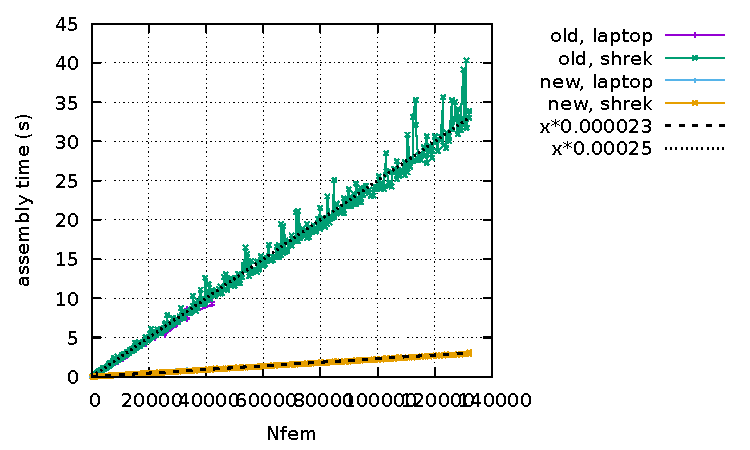
\includegraphics[width=8.5cm]{images/oneD/assembly}
\end{center}
The assembled matrix and rhs are then (I have dropped the $new$ superscripts):
\[
\left(
\begin{array}{ccccc}
A_{00}^{{\color{red}\tt 0}} &  A_{01}^{{\color{red}\tt 0}} &0&0&0 \\ \\ 
A_{10}^{{\color{red}\tt 0}} &  A_{11}^{{\color{red} \tt 0}} \!+\! A_{00}^{{\color{red}\tt 1}}  & A_{01}^{{\color{red}\tt 1}}   &0&0 \\ \\
0& A_{10}^{{\color{red}\tt 1}} & A_{11}^{{\color{red} \tt 1}} \! +\! A_{00}^{{\color{red}\tt 2}}  & A_{01}^{{\color{red}\tt 2}}   & 0\\ \\
0&0& A_{10}^{{\color{red}\tt 2}}   & A_{11}^{{\color{red}\tt 2}} \! +\! A_{00}^{{\color{red}\tt 3}}   & A_{01}^{{\color{red}\tt 3}}  \\ \\
0&0&0& A_{10}^{{\color{red}\tt 3}}   & A_{11}^{{\color{red}\tt 3}} 
\end{array}
\right)
\left(
\begin{array}{c}
T_0 \\\\ T_1 \\\\ T_2 \\\\ T_3 \\\\ T_4
\end{array}
\right)
=
\left(
\begin{array}{c}
b_{0}^{{\color{red}\tt 0}} \\ \\
b_{1}^{{\color{red}\tt 0}} + b_{0}^{{\color{red}\tt 1}}\\ \\
b_{1}^{{\color{red}\tt 1}} + b_{0}^{{\color{red}\tt 2}}\\ \\
b_{1}^{{\color{red}\tt 2}} + b_{0}^{{\color{red}\tt 3}}\\ \\
b_{1}^{{\color{red}\tt 3}} 
\end{array}
\right)
\]
Ultimately the assembled matrix system also takes the form
\[
\left(
\begin{array}{ccccc}
{\cal A}_{00} & {\cal A}_{01} & 0& 0& 0\\ \\
{\cal A}_{10} & {\cal A}_{11} & {\cal A}_{12}& 0 & 0\\\\
0 & {\cal A}_{21} & {\cal A}_{22}&  {\cal A}_{23}  & 0\\\\
0&0&   {\cal A}_{32} & {\cal A}_{33}&  {\cal A}_{34} \\\\
0&0&0   & {\cal A}_{43}&  {\cal A}_{44} \\\\
\end{array}
\right)
\left(
\begin{array}{c}
T_0 \\\\ T_1 \\\\ T_2 \\\\ T_3 \\\\ T_4
\end{array}
\right)
=
\left(
\begin{array}{c}
b_0\\\\
b_1\\\\
b_2\\\\
b_3\\\\
b_4
\end{array}
\right)
\]
and we see that it is sparse. Its sparsity structure is easy to derive: each row corresponds to a dof, 
and since nodes 1 and 2 'see' each other (they belong to the same element) there will be non-zero entries
in the first and second column. 
Likewise, node 2 'sees' node 1 (in other words, there is an edge linking nodes 1 and 2), itself, 
and node 3, so that there are non-zero entries in the second row at columns 1, 2, and 3.

Before we solve the system, we need to take care of boundary conditions.
Let us assume that we wish to fix the temperature at node 2, or in other words 
we wish to set 
\[
T_2 = T^{o}
\]
This equation can be cast as
\[
\left(
\begin{array}{ccccc}
 0 & 1 & 0 & 0 & 0
\end{array}
\right)
\left(
\begin{array}{c}
T_1 \\ T_2 \\ T_3 \\ T_4 \\ T_5
\end{array}
\right)
=
\left(
\begin{array}{c}
0 \\
T^{o} \\
0 \\
0 \\
0
\end{array}
\right)
\]

This replaces the second line in the previous matrix equation:
\[
\left(
\begin{array}{ccccc}
{\cal A}_{11} & {\cal A}_{12} & 0& 0& 0\\ \\
0 & 1 & 0 & 0 & 0 \\ \\
0 & {\cal A}_{32} & {\cal A}_{33}&  {\cal A}_{34} & 0 \\\\
0&0&   {\cal A}_{43} & {\cal A}_{44}&  {\cal A}_{45} \\\\
0&0&0   & {\cal A}_{54}&  {\cal A}_{55} \\\\
\end{array}
\right)
\left(
\begin{array}{c}
T_1 \\\\ T_2 \\\\ T_3 \\\\ T_4 \\\\ T_5
\end{array}
\right)
=
\left(
\begin{array}{c}
b_{1} \\ \\
T^{o} \\ \\
b_{3}\\\\
b_{4}\\\\
b_{5}
\end{array}
\right)
\]
That's it, we have a linear system of equations which can be solved!


The following figure presents a hand-drawn template of how 
a typical 1D FE code is structured:
\begin{center}
\includegraphics[width=16cm]{images/fem_exercises/FEMcode_structure}\\
{\captionfont Additional comments: A and b should be zeroed at every time step.
Convergence should be tested before Told received T.}
\end{center}




%-/-/-/-/-/-/-/-/-/-/-/-/-/-/-/-/-/-/
\begin{center}
\begin{minipage}[t]{0.77\textwidth}
\par\noindent\rule{\textwidth}{0.4pt}

\begin{center}
\includegraphics[width=0.8cm]{images/garftr} \\
{\color{orange}Exercise FEM-01}
\end{center}

Write a code which solves the 1D diffusion equation in time. 
The initial temperature field is as follows:
\begin{center}
\includegraphics[width=6cm]{images/fem_exercises/tempinit}
\end{center}
\[
T(x,t=0)=200 \quad x<L_x/2
\quad\quad\quad
T(x,t=0)=100 \quad x\geq L_x/2
\]

The domain is $L_x=100$km and the properties of the material are 
$\rho=3000kg/m^3$, $k=3W/m/K$, $C_p=1000J/K$.
Boundary conditions are:
\[
T(t,x=0)=200^\circ C
\quad\quad
T(t,x=L_x)=100^\circ C
\]
There are {\tt nelx} elements and {\tt nnx} nodes.
All elements are {\tt hx} long.
The code will carry out {\tt nstep} timesteps of length {\tt dt}
with 
$\delta t = 0.5 \frac{h^2_x}{\kappa}$.

Bonus: add a small random perturbation up to $\pm$20\% of $h_x$ to each node position 
inside the domain and make sure that the recovered steady state solution is unchanged.

\par\noindent\rule{\textwidth}{0.4pt}
\end{minipage}
\end{center}

